\subsection{Condiciones experimentales}

Los resultados que siguen se obtuvieron con la configuración de PSO de la
Tabla~\ref{tab:m2_parametros} (Sección~\ref{sec:parametrizacion}), sobre las 9 instancias
de la Tabla~\ref{tab:m2_instancias}, con 31 repeticiones independientes por
instancia (semillas $0,\ldots,30$) y un presupuesto de $50\,000$ evaluaciones de la
función objetivo por corrida. Se registran, por instancia: el costo de la mejor solución
encontrada, el costo promedio y su desviación estándar sobre las 31 corridas, el GAP\,\%
respecto al óptimo o BKS de la Tabla~\ref{tab:m2_instancias}, y el tiempo de ejecución
promedio por corrida. El entorno de ejecución se describe en la
Sección~\ref{sec:parametrizacion} (equipo personal, Python/NumPy/Numba/Optuna).

\subsection{Resultados del método PSO}

La Tabla~\ref{tab:m2_resultados_pso} resume el desempeño de PSO sobre las 9 instancias
evaluadas.

\begin{table}[H]
\centering
\caption{Resultados de PSO sobre instancias de CVRPLIB. Estadísticos sobre 31 repeticiones
independientes por instancia. Ref.\ es el óptimo certificado o BKS de la
Tabla~\ref{tab:m2_instancias}; las últimas cuatro filas (bajo la línea) corresponden a
instancias fuera del alcance del método exacto.}
\label{tab:m2_resultados_pso}
\begin{tabular}{lrrrrrrr}
\hline
Instancia & $n$ & Ref.\ & Mejor & Prom. & Desv. & Gap prom.\ (\%) & Tiempo (s) \\
\hline
E-n13-k4  & 13  & 247  & 251  & 256{,}6  & 3{,}0  & 3{,}89  & 0{,}066 \\
E-n22-k4  & 22  & 375  & 376  & 392{,}5  & 12{,}3 & 4{,}66  & 0{,}086 \\
E-n23-k3  & 23  & 569  & 569  & 569{,}2  & 0{,}4  & 0{,}03  & 0{,}096 \\
A-n32-k5  & 32  & 784  & 786  & 816{,}7  & 25{,}4 & 4{,}17  & 0{,}106 \\
A-n33-k5  & 33  & 661  & 697  & 727{,}6  & 16{,}2 & 10{,}07 & 0{,}106 \\
\hline
A-n60-k9   & 60  & 1354 & 1486 & 1560{,}5 & 56{,}3 & 15{,}25 & 0{,}172 \\
E-n76-k10  & 76  & 830  & 924  & 1013{,}2 & 40{,}3 & 22{,}07 & 0{,}212 \\
A-n80-k10  & 80  & 1763 & 1911 & 2045{,}4 & 71{,}3 & 16{,}02 & 0{,}226 \\
E-n101-k8  & 101 & 815  & 954  & 1033{,}7 & 44{,}2 & 26{,}84 & 0{,}306 \\
\hline
\end{tabular}
\end{table}

En cuatro de las cinco instancias compartidas con el método exacto ($n\le33$), PSO se
mantiene por debajo del $5\%$ de GAP promedio, e incluso alcanza el óptimo exacto en
\texttt{E-n23-k3}; la excepción es \texttt{A-n33-k5} ($10{,}07\%$). En las cuatro
instancias adicionales ($n\ge60$), el GAP promedio se mueve entre $15{,}25\%$ y
$26{,}84\%$, con una tendencia creciente respecto del tamaño que no es estrictamente
monótona: \texttt{E-n76-k10} ($22{,}07\%$) supera a \texttt{A-n80-k10} ($16{,}02\%$)
pese a ser más chica, lo que indica que la dificultad no depende solo de $n$ sino
también de la estructura de cada instancia (la razón demanda/capacidad y el número de
vehículos difieren entre ambas familias). La Figura~\ref{fig:m2_boxplot_gap} (construida
a partir de los mismos datos de la tabla) muestra este patrón mediante la distribución
completa del GAP\,\% de las 31 corridas por instancia, no solo su promedio.

\begin{figure}[H]
    \centering
    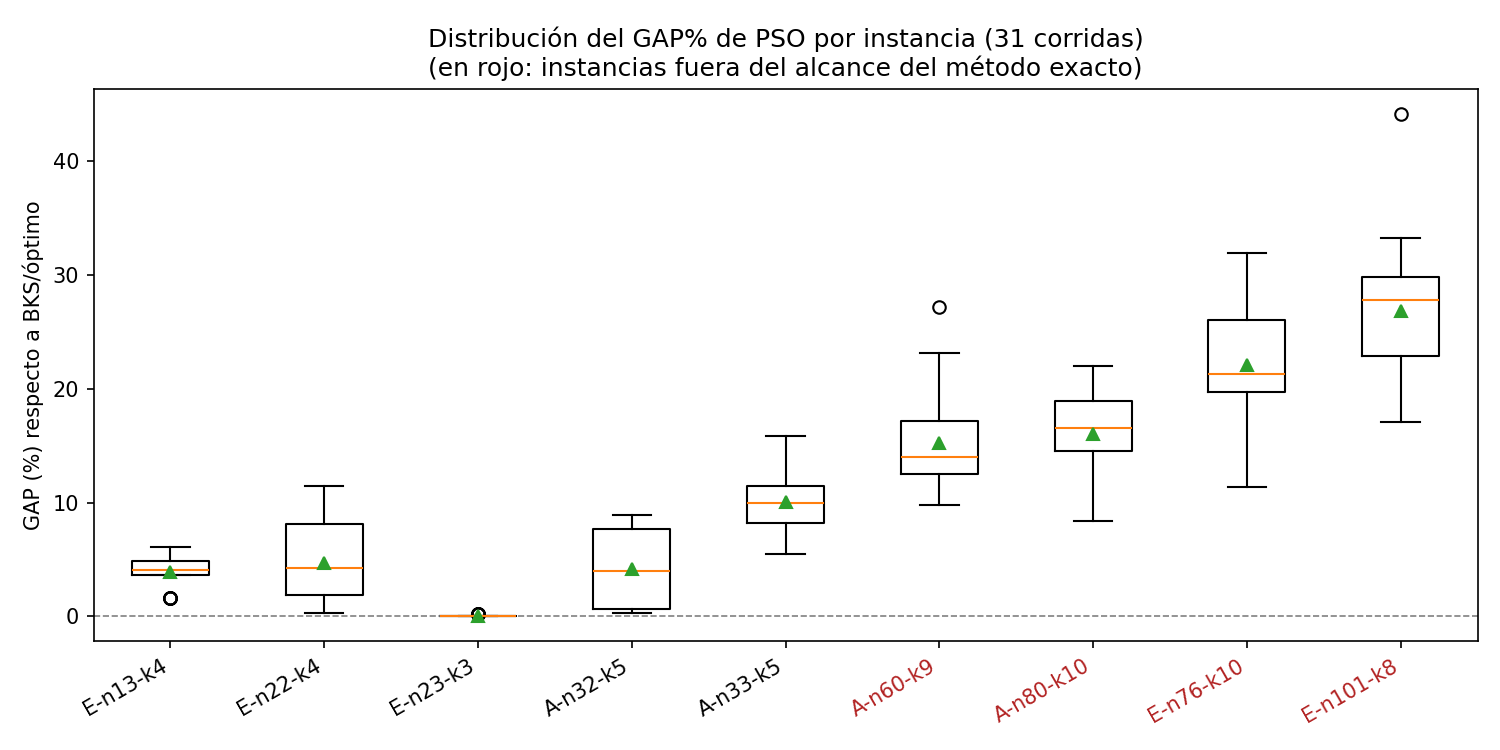
\includegraphics[width=0.85\textwidth]{figuras/boxplot_gap_pso.png}
    \caption{Distribución del GAP\,\% de PSO por instancia (31 corridas). En rojo, las
    cuatro instancias fuera del alcance del método exacto. Fuente: elaboración propia.}
    \label{fig:m2_boxplot_gap}
\end{figure}

La tendencia creciente del GAP con el tamaño es consistente con lo observado ya en la
parametrización (Sección~\ref{sec:parametrizacion}): las instancias de tuning más grandes
(\texttt{A-n62-k8}, GAP $7{,}92\%$; \texttt{E-n76-k7}, GAP $14{,}37\%$) también mostraron
GAP mayor que la chica (\texttt{A-n34-k5}, GAP $3{,}34\%$). Además, las dos instancias de
evaluación más grandes ($n=80$ y $n=101$) exceden el tamaño de la mayor instancia de
tuning usada ($n=76$), por lo que en ese rango los parámetros operan fuera de la escala
en que fueron calibrados; se retoma esta observación en la discusión.

\subsection{Análisis de convergencia}

La Figura~\ref{fig:m2_convergencia} muestra la evolución del GAP\,\% del mejor global del
enjambre en función de la iteración, para una instancia chica compartida con el método
exacto (\texttt{A-n32-k5}, $n=32$) y la instancia más grande del conjunto de evaluación
(\texttt{E-n101-k8}, $n=101$). La línea es la corriente mediana de las 31 repeticiones; la
banda sombreada es el rango entre la mejor y la peor corrida en cada iteración.

\begin{figure}[H]
    \centering
    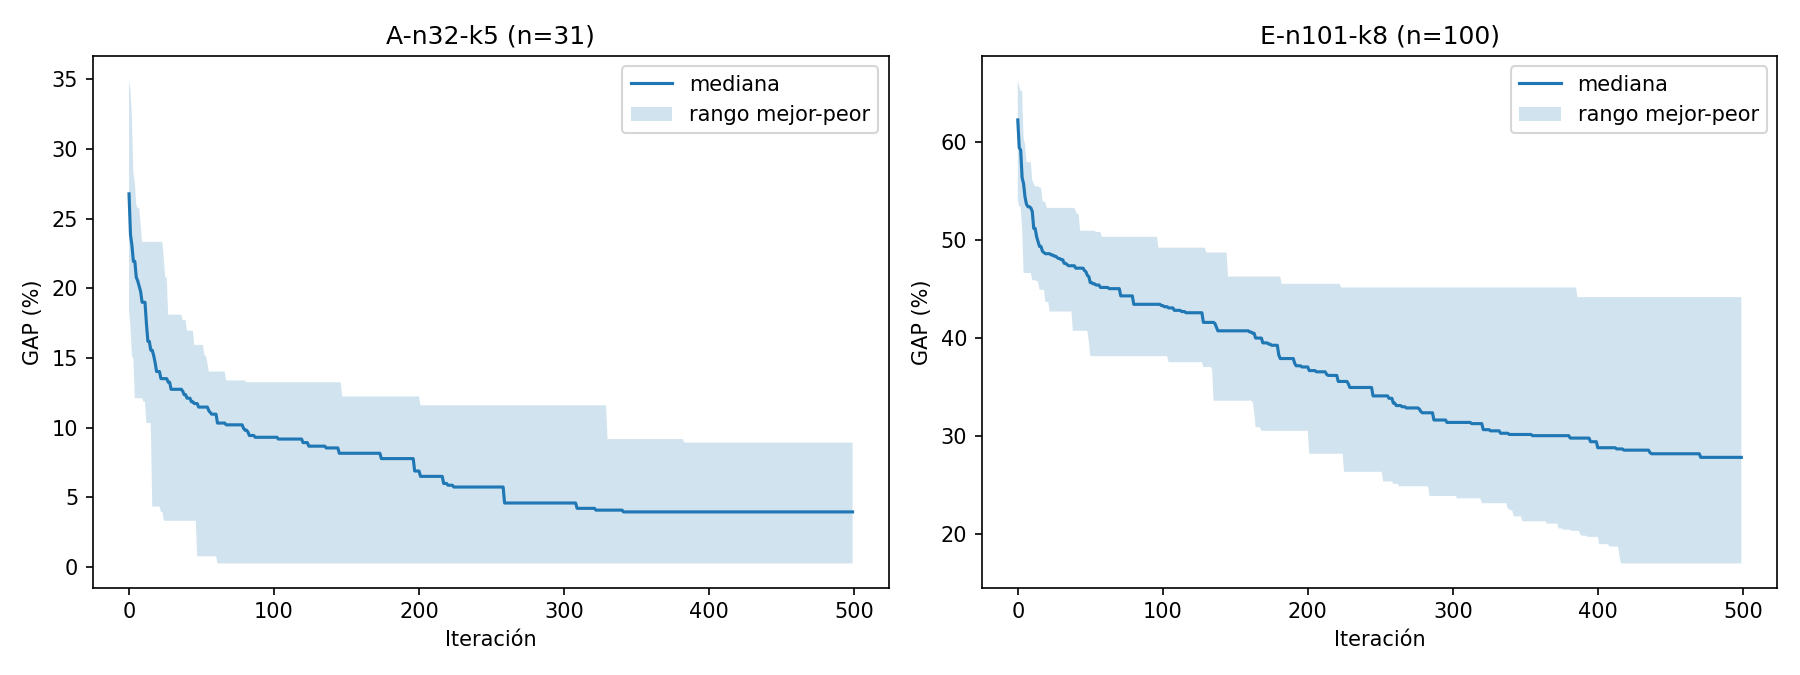
\includegraphics[width=0.95\textwidth]{figuras/convergencia_comparacion.png}
    \caption{Curvas de convergencia de PSO (GAP\,\% vs.\ iteración) para una instancia
    chica (\texttt{A-n32-k5}) y una grande (\texttt{E-n101-k8}). Línea: mediana de 31
    corridas; banda: rango mejor-peor. Fuente: elaboración propia.}
    \label{fig:m2_convergencia}
\end{figure}

En \texttt{A-n32-k5}, la última mejora de la curva mediana ocurre en la iteración 341 de
las 500 disponibles (Tabla~\ref{tab:m2_parametros}): el último tercio de la corrida
transcurre sin cambios en la mediana, es decir, el enjambre agota su margen de mejora
antes de agotar su presupuesto de iteraciones. En \texttt{E-n101-k8}, en cambio, la
mediana sigue mejorando hasta prácticamente el final (última mejora en la iteración 471
de 500), y su descenso aún es visible en el tramo final de la curva: el mismo presupuesto
que sobra en la instancia chica apenas alcanza en la más grande. Dado que $T$ se deriva
de un presupuesto fijo de evaluaciones igual para todas las instancias
($T=\lfloor 50\,000/N\rfloor$, Sección~\ref{sec:parametrizacion}), las instancias de
mayor dimensión de búsqueda ($n+2m$ crece con $n$) disponen relativamente de menos
iteraciones para explorar un espacio más grande, lo que contribuye al mayor GAP
observado en la Tabla~\ref{tab:m2_resultados_pso} para $n\ge60$, más allá de la calidad
de la parametrización misma.

\subsection{Comparación con el método exacto}
\label{sec:m2_comparacion}

La Tabla~\ref{tab:m2_comparacion} contrasta el método exacto del Informe~1 con PSO sobre
las cinco instancias comunes. Esta comparación constituye el objetivo central del informe
(requisito~8 del enunciado).

\begin{table}[H]
\centering
\caption{Comparación método exacto (Informe~1) vs.\ PSO, sobre las cinco instancias
compartidas. Gap de PSO respecto al óptimo o BKS de la Tabla~\ref{tab:m2_instancias}
(661 en \texttt{A-n33-k5}, no 667). Tiempo de PSO: promedio de 31 corridas.}
\label{tab:m2_comparacion}
\begin{tabular}{lrrrrrr}
\hline
 & \multicolumn{3}{c}{Exacto (Informe 1)} & \multicolumn{3}{c}{PSO (mejor de 31)} \\
\cmidrule(lr){2-4}\cmidrule(lr){5-7}
Instancia & $z^{*}$ & Gap (\%) & Tiempo (s) & Mejor & Gap (\%) & Tiempo (s) \\
\hline
E-n13-k4  & 247 & 0{,}00 & 0{,}9       & 251 & 1{,}62 & 0{,}066 \\
E-n22-k4  & 375 & 0{,}00 & 0{,}8       & 376 & 0{,}27 & 0{,}086 \\
E-n23-k3  & 569 & 0{,}00 & 1{,}2       & 569 & 0{,}00 & 0{,}096 \\
A-n32-k5  & 784 & 0{,}00 & 576{,}1     & 786 & 0{,}26 & 0{,}106 \\
A-n33-k5  & 667 & 0{,}91 & 17\,096{,}4 & 697 & 5{,}45 & 0{,}106 \\
\hline
\end{tabular}
\end{table}

En las instancias más chicas ($n\le23$), ambos métodos son prácticamente instantáneos
(menos de 1{,}2~s el exacto, menos de 0{,}1~s PSO) y PSO queda a menos de $2\%$ del
óptimo. A partir de $n=32$ la brecha de tiempo se abre por completo: el exacto pasa de
$1{,}2$~s en \texttt{E-n23-k3} a $576{,}1$~s en \texttt{A-n32-k5} y a $17\,096{,}4$~s
($4{,}7$~h) en \texttt{A-n33-k5}, sin siquiera certificar optimalidad en esta última
(Tabla~\ref{tab:m2_instancias}); PSO, en cambio, se mantiene en $0{,}1$~s en ambas,
sin variación apreciable. La razón de tiempos entre PSO y el exacto es de
aproximadamente $5\,460\times$ en \texttt{A-n32-k5} y $161\,000\times$ en
\texttt{A-n33-k5}: una diferencia de varios órdenes de magnitud, medida en el mismo
equipo para ambos métodos (Sección~\ref{sec:parametrizacion}), por lo que no es
atribuible a ninguna diferencia de infraestructura.

La Figura~\ref{fig:m2_convergencia_tiempo} presenta esta misma comparación de forma
gráfica: la curva de convergencia de PSO en función del tiempo real (no de iteraciones),
en escala logarítmica, junto con el resultado final del método exacto representado como
un único punto, ya que este último no dispone de una curva de convergencia comparable en
esta comparación (no se re-ejecutó para registrar su incumbente por iteración).

\begin{figure}[H]
    \centering
    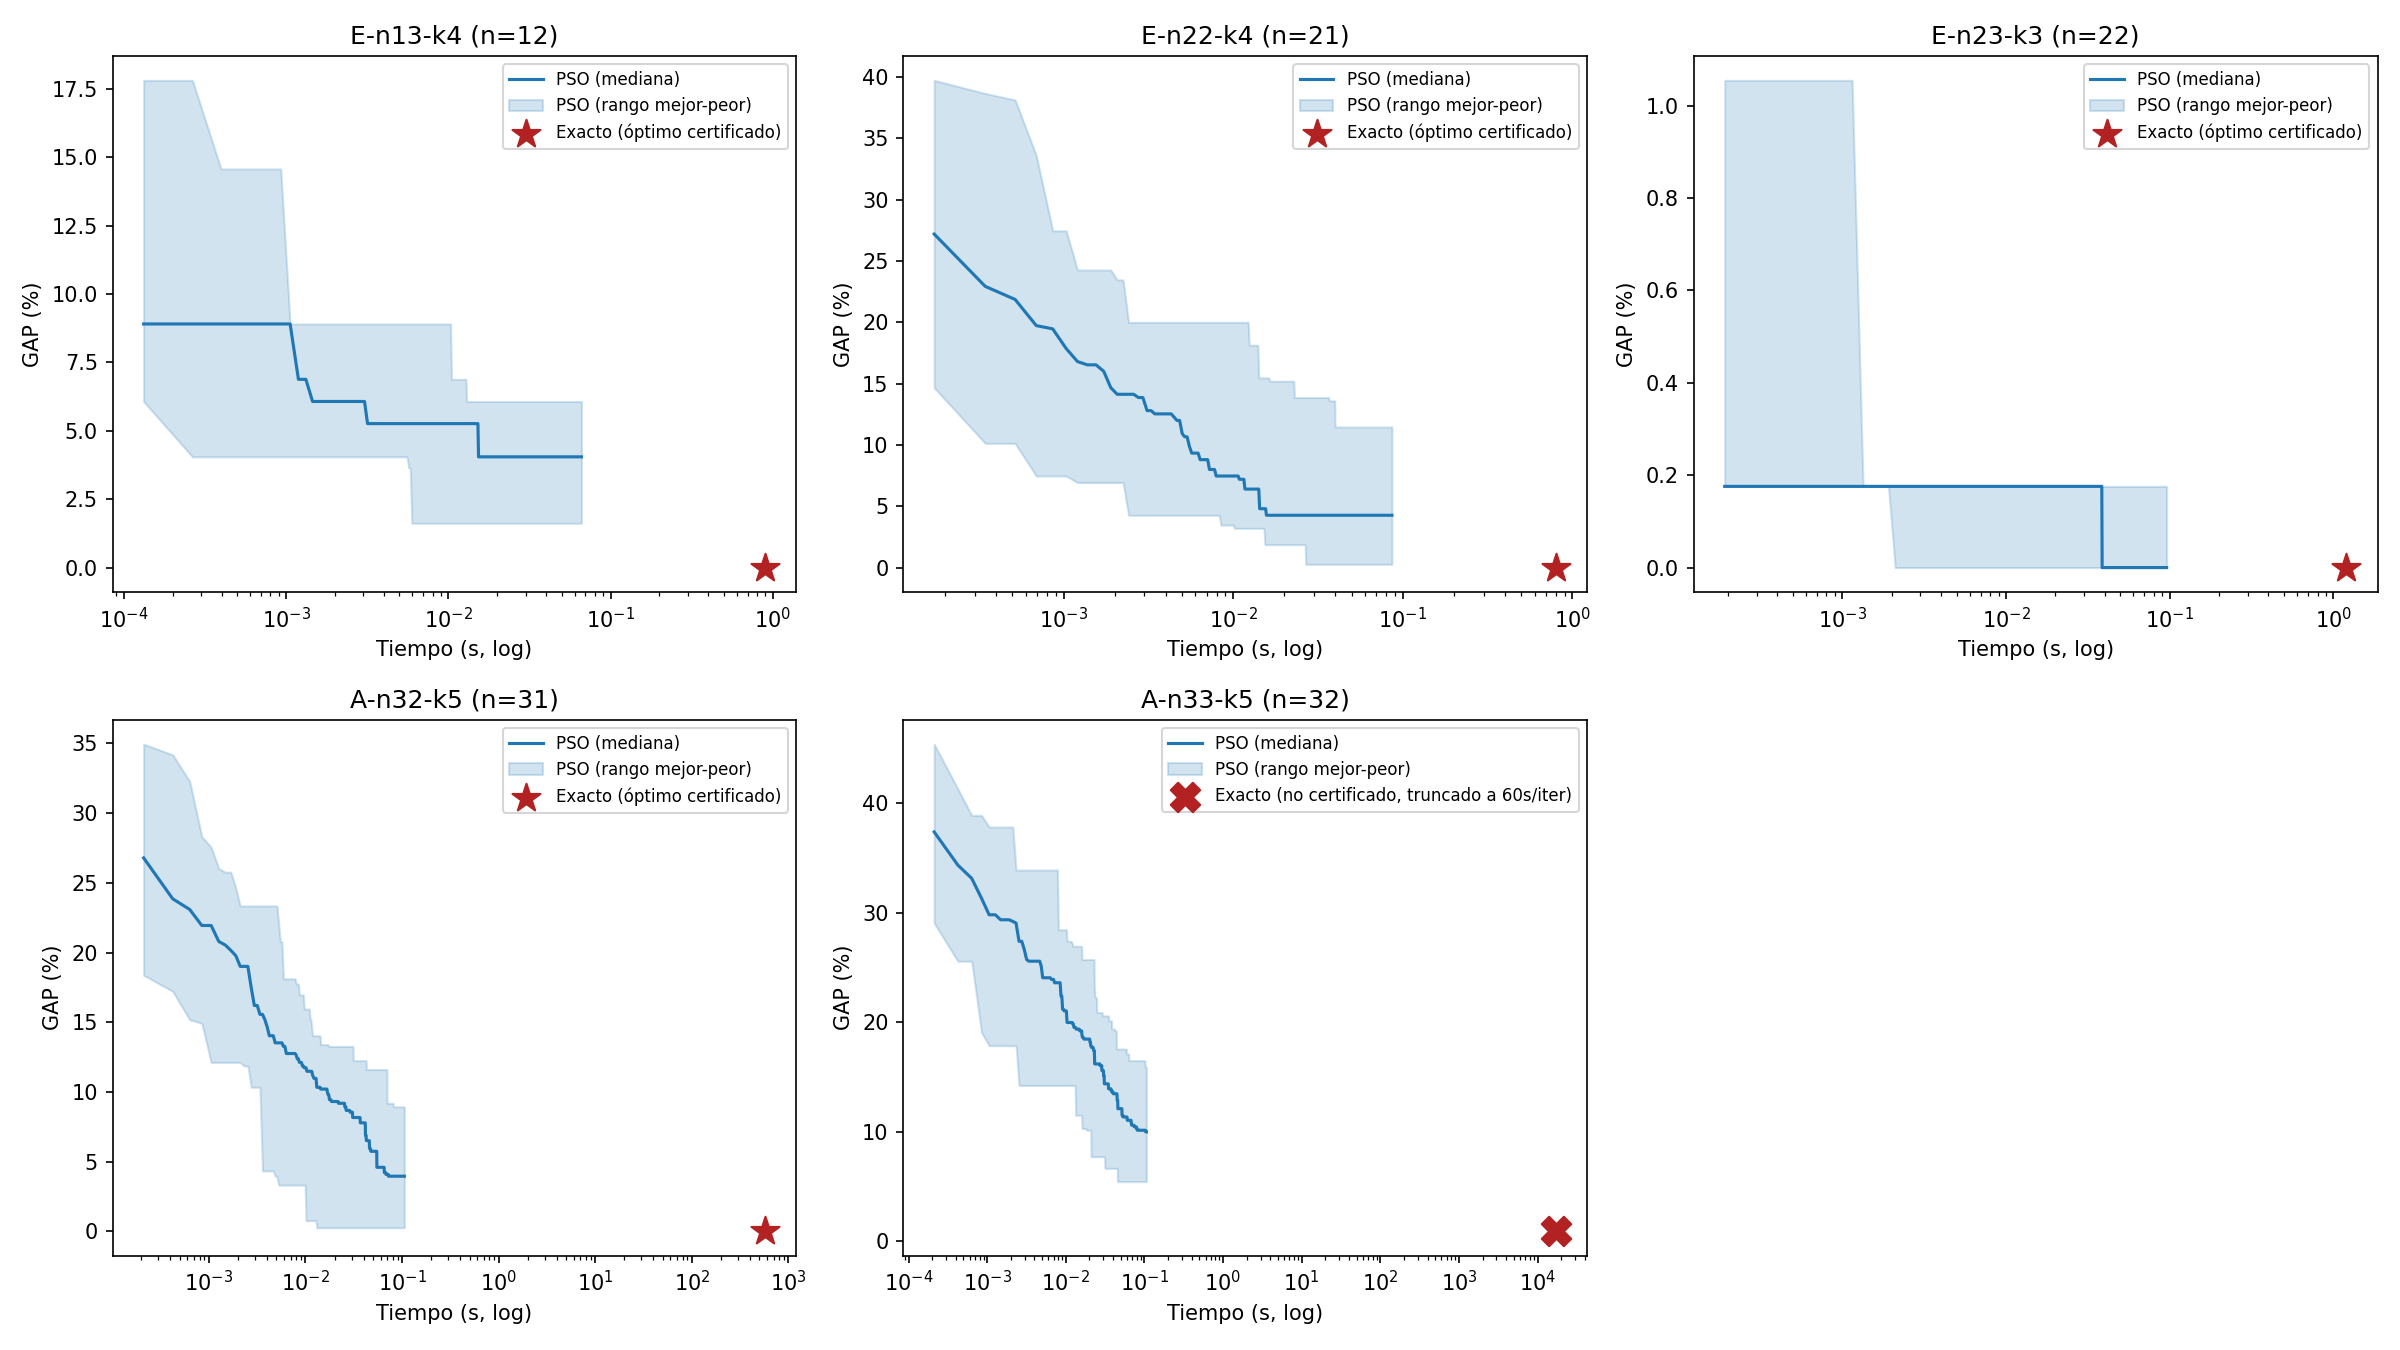
\includegraphics[width=0.95\textwidth]{figuras/convergencia_tiempo_exacto_vs_pso.png}
    \caption{Convergencia de PSO en tiempo real (escala log) para las cinco instancias
    compartidas con el método exacto. El punto rojo marca el resultado final del método
    exacto (estrella: óptimo certificado; cruz: no certificado, truncado por el límite de
    60\,s por resolución del modelo entero). Fuente: elaboración propia.}
    \label{fig:m2_convergencia_tiempo}
\end{figure}

El punto queda siempre muy a la derecha del tramo donde la curva de PSO ya se aplanó,
ilustrando visualmente el mismo hallazgo de la Tabla~\ref{tab:m2_comparacion}: PSO
alcanza su mejor solución en una fracción de segundo, mientras el exacto necesita órdenes
de magnitud más tiempo para llegar a un punto (certificado o no) que, en el peor caso
observado (\texttt{A-n33-k5}), PSO iguala o incluso mejora en calidad relativa apenas
$5{,}45\%$ por encima del óptimo real, en una fracción del tiempo.
